\documentclass[tikz,border=10pt]{standalone}
\usepackage{tikz}
\usetikzlibrary{shapes,patterns,positioning}
\usetikzlibrary{angles, quotes, positioning, arrows.meta, decorations.markings}
\begin{document}
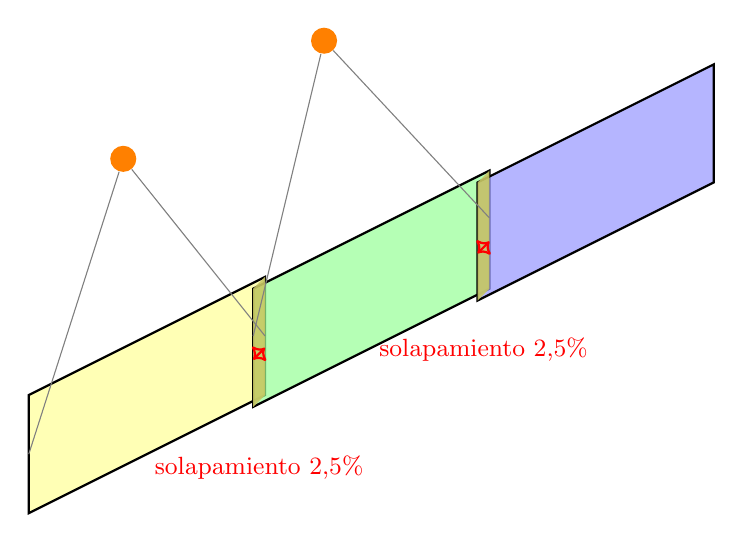
\begin{tikzpicture}[scale=1.5]
    % Definir colores para diferentes swaths
    \definecolor{swath1}{RGB}{255,255,150}  % Amarillo claro
    \definecolor{swath2}{RGB}{150,255,150}  % Verde claro
    \definecolor{swath3}{RGB}{150,150,255}  % Azul claro
    \definecolor{overlap}{RGB}{200,200,100} % Color de solapamiento
    
    
    % Primer swath
    \fill[swath1, opacity=0.7] (0,0.5) -- (2,1.5) -- (2,2.5) -- (0,1.5) -- cycle;
    \draw[thick] (0,0.5) -- (2,1.5) -- (2,2.5) -- (0,1.5) -- cycle;
    
    % Segundo swath con 5% de solapamiento
    \fill[swath2, opacity=0.7] (1.9,1.4) -- (3.9,2.4) -- (3.9,3.4) -- (1.9,2.4) -- cycle;
    \draw[thick] (1.9,1.4) -- (3.9,2.4) -- (3.9,3.4) -- (1.9,2.4) -- cycle;
    
    % Tercer swath con 5% de solapamiento
    \fill[swath3, opacity=0.7] (3.8,2.3) -- (5.8,3.3) -- (5.8,4.3) -- (3.8,3.3) -- cycle;
    \draw[thick] (3.8,2.3) -- (5.8,3.3) -- (5.8,4.3) -- (3.8,3.3) -- cycle;
    
    % Marcar zonas de solapamiento
    \fill[overlap, opacity=0.9] (1.9,1.4) -- (2,1.5) -- (2,2.5) -- (1.9,2.4) -- cycle;
    \fill[overlap, opacity=0.9] (3.8,2.3) -- (3.9,2.4) -- (3.9,3.4) -- (3.8,3.3) -- cycle;
    
    % Satélites en órbitas
    \node[circle, fill=orange, minimum size=8pt] (sat1) at (0.8,3.5) {};
    \node[circle, fill=orange, minimum size=8pt] (sat2) at (2.5,4.5) {};

    
    % Líneas de vista desde satélites
    \draw[thin, gray] (sat1) -- (0,1);
    \draw[thin, gray] (sat1) -- (2,2);
    \draw[thin, gray] (sat2) -- (1.9,2);
    \draw[thin, gray] (sat2) -- (3.9,3);
    
    % Indicar porcentaje de solapamiento
    \draw[<->, red, thick] (1.9,1.8) -- (2,1.9);
    \node[red, above] at (1.95,0.7) {\small solapamiento 2,5\%};
    
    \draw[<->, red, thick] (3.8,2.7) -- (3.9,2.8);
    \node[red, above] at (3.85,1.7) {\small solapamiento 2,5\%};
    
\end{tikzpicture}

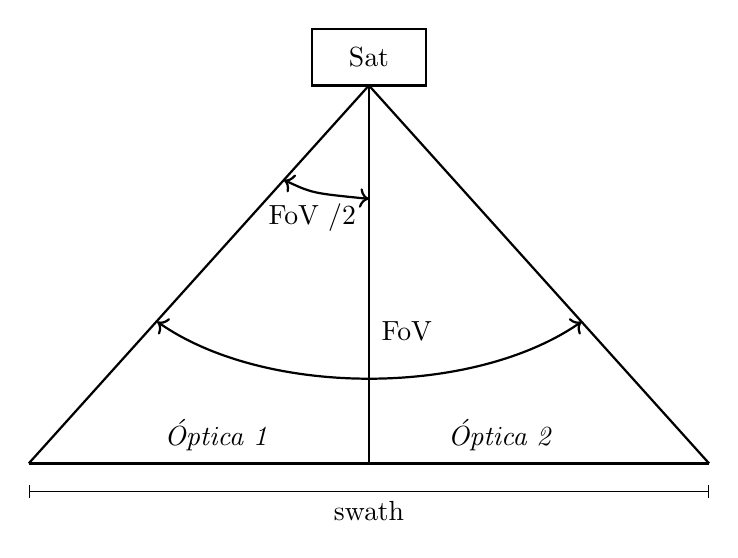
\begin{tikzpicture}[scale=1.2]

% Satélite
\draw[thick] (0,4) rectangle (1.2,4.6);
\node at (0.6,4.3) {Sat};

% Línea central
\draw[thick] (0.6,4) -- (0.6,0);

% Pirámide de visión
\draw[thick] (0.6,4) -- (-3,0);
\draw[thick] (0.6,4) -- (4.2,0);

% Línea base (swath)
\draw[thick] (-3,0) -- (4.2,0);

% Etiqueta de swath
\draw[|-|] (-3,-0.3) -- (4.2,-0.3);
\node at (0.6,-0.5) {swath};

% Ángulo FoV
\draw[<->,thick] (-0.3,3) .. controls (-0,2.86)  .. (0.6,2.8);
\node at (-0.0,2.6) {FoV /2};

% Ángulo FoVx2
\draw[<->,thick] (-1.64,1.5) .. controls (-0.5,0.7) and (1.7,0.7) .. (2.85,1.5);
\node at (1,1.4) {FoV};

% Etiquetas adicionales
\node at (2.5,2) { };
\node at (-1.0,0.3) {\textit{Óptica 1}};
\node at (2.0,0.3) {\textit{Óptica 2}};
\end{tikzpicture}


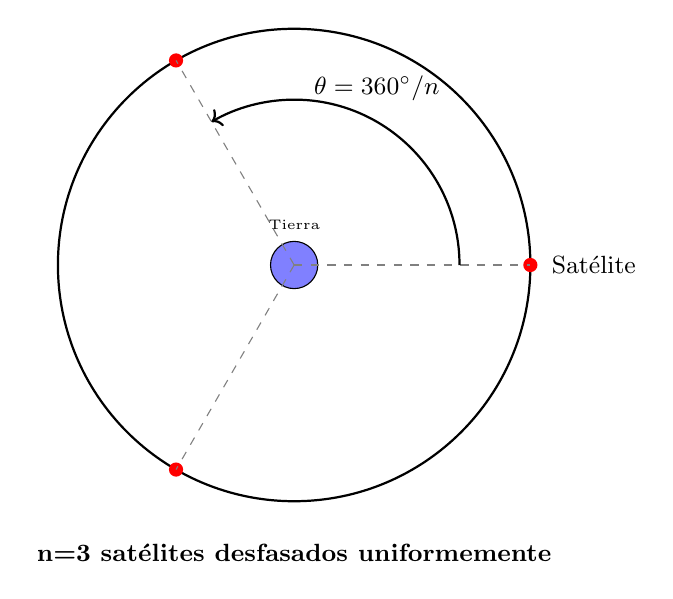
\begin{tikzpicture}[scale=3]

% Dibuja la órbita
\draw[thick] (0,0) circle (1);

% Dibuja la Tierra
\filldraw[fill=blue!50] (0,0) circle (0.1);
\node at (0,0.17) {\tiny Tierra};

% Satélites (n=3) y líneas angulares
\foreach \i in {0,1,2} {
    % Posición del satélite
    \coordinate (S\i) at ({cos(120*\i)},{sin(120*\i)});
    % Satélite como punto rojo
    \fill[red] (S\i) circle (0.03);
    % Línea discontinua del centro al satélite
    \draw[dashed,gray] (0,0) -- (S\i);
}

% Arco para indicar el ángulo theta
\draw[->,thick] (0.7,0) arc (0:120:0.7);
\node at ({0.7*cos(60)},{0.7*sin(60)+0.14}) {\small $\theta = 360^\circ/n$};

% Texto explicativo
\node at (0,-1.22) {\small \textbf{n=3 satélites desfasados uniformemente}};

% Leyenda en recuadro


    \node[right] at (1.05,0) {\small Satélite};


\end{tikzpicture}

\begin{tikzpicture}
    % 1. Cargar la imagen como un nodo base
    \node[anchor=south west, inner sep=0] (image) at (0,0) 
        {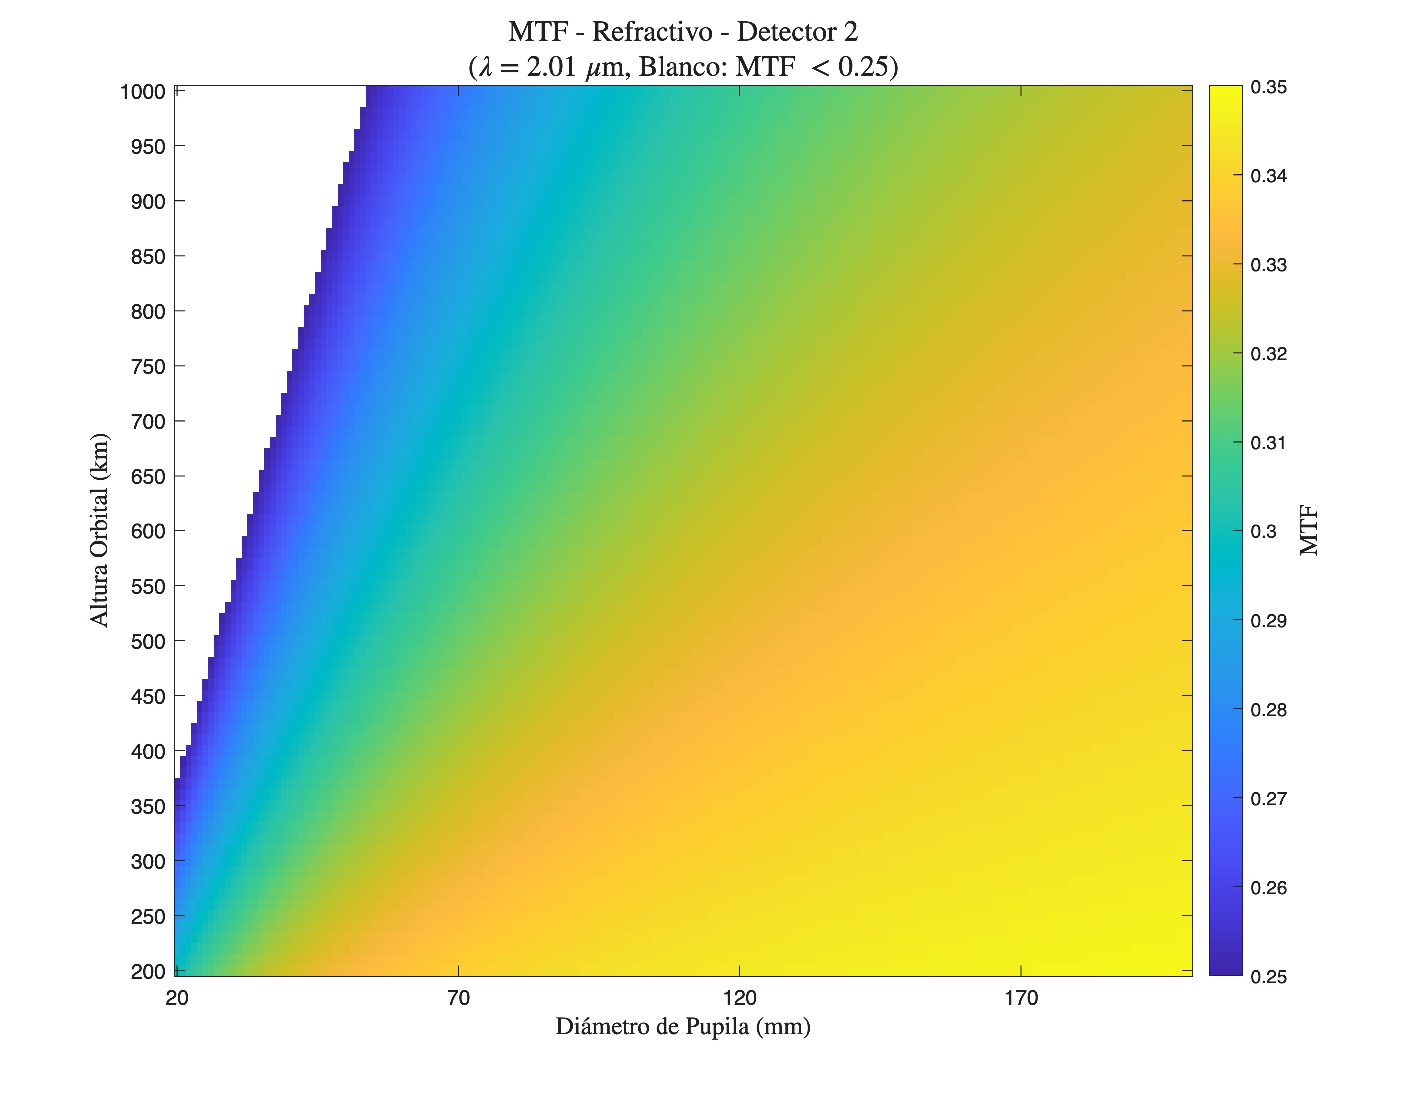
\includegraphics[width=12cm]{mtf_selected_heatmap.pdf}};

    % 2. Definir un sistema de coordenadas relativo a la imagen para facilitar la colocación
    %    El origen (0,0) es la esquina inferior izquierda.
    %    El punto (1,1) es la esquina superior derecha.
    \begin{scope}[x={(image.south east)}, y={(image.north west)}]

        
        \coordinate (PuntoDiseno) at (0.18, 0.54);

        % 4. Dibujar el punto rojo en las coordenadas definidas
        \fill[red] (PuntoDiseno) circle (2pt);

        % 5. Crear la caja de texto (label) y una flecha apuntando al punto
        %    El nodo se posiciona relativo al punto para que sea fácil de mover.
        \node[fill=white, draw, thick, anchor=south west, inner sep=2pt] (label) 
            at ([xshift=10pt, yshift=10pt]PuntoDiseno) {Punto de diseño};
            
        % Dibuja una línea/flecha desde la caja de texto al punto
        \draw[->, thick, -latex] (label.south west) -- (PuntoDiseno);

    \end{scope}
\end{tikzpicture}

\begin{tikzpicture}
    % 1. Cargar la imagen como un nodo base
    \node[anchor=south west, inner sep=0] (image) at (0,0) 
        {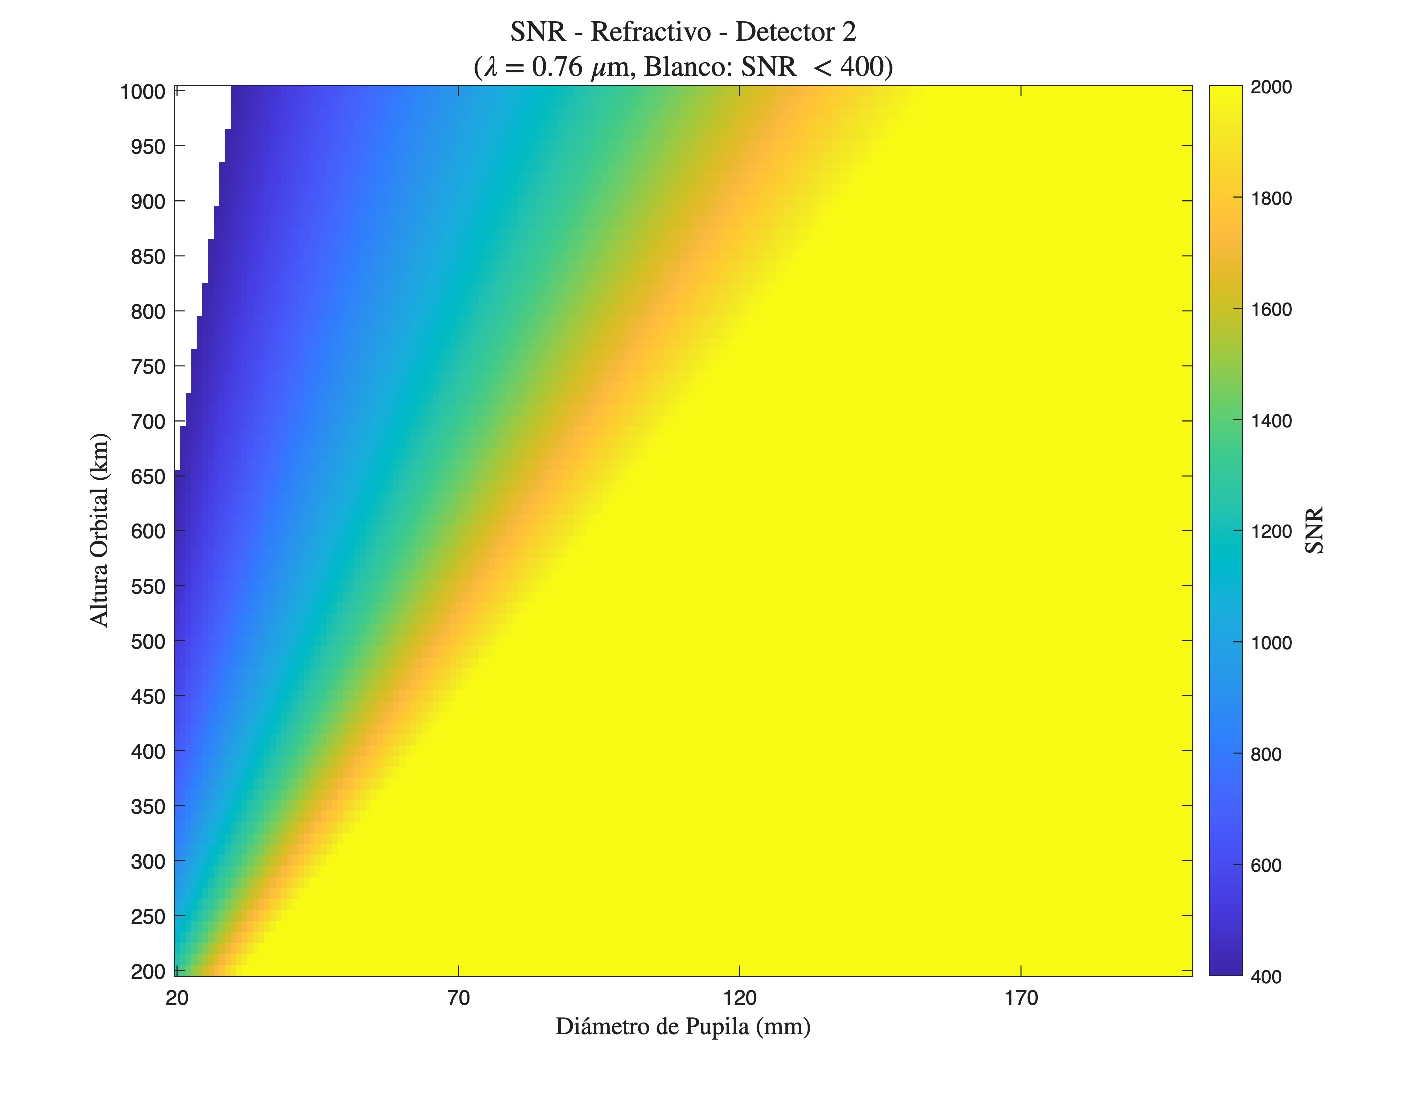
\includegraphics[width=12cm]{snr_selected_heatmap.pdf}};

    % 2. Definir un sistema de coordenadas relativo a la imagen para facilitar la colocación
    %    El origen (0,0) es la esquina inferior izquierda.
    %    El punto (1,1) es la esquina superior derecha.
    \begin{scope}[x={(image.south east)}, y={(image.north west)}]

        
        \coordinate (PuntoDiseno) at (0.18, 0.54);

        % 4. Dibujar el punto rojo en las coordenadas definidas
        \fill[red] (PuntoDiseno) circle (2pt);

        % 5. Crear la caja de texto (label) y una flecha apuntando al punto
        %    El nodo se posiciona relativo al punto para que sea fácil de mover.
        \node[fill=white, draw, thick, anchor=south west, inner sep=2pt] (label) 
            at ([xshift=10pt, yshift=10pt]PuntoDiseno) {Punto de diseño};
            
        % Dibuja una línea/flecha desde la caja de texto al punto
        \draw[->, thick, -latex] (label.south west) -- (PuntoDiseno);

    \end{scope}
\end{tikzpicture}

\begin{tikzpicture}
    % 1. Cargar la imagen como un nodo base
    \node[anchor=south west, inner sep=0] (image) at (0,0) 
        {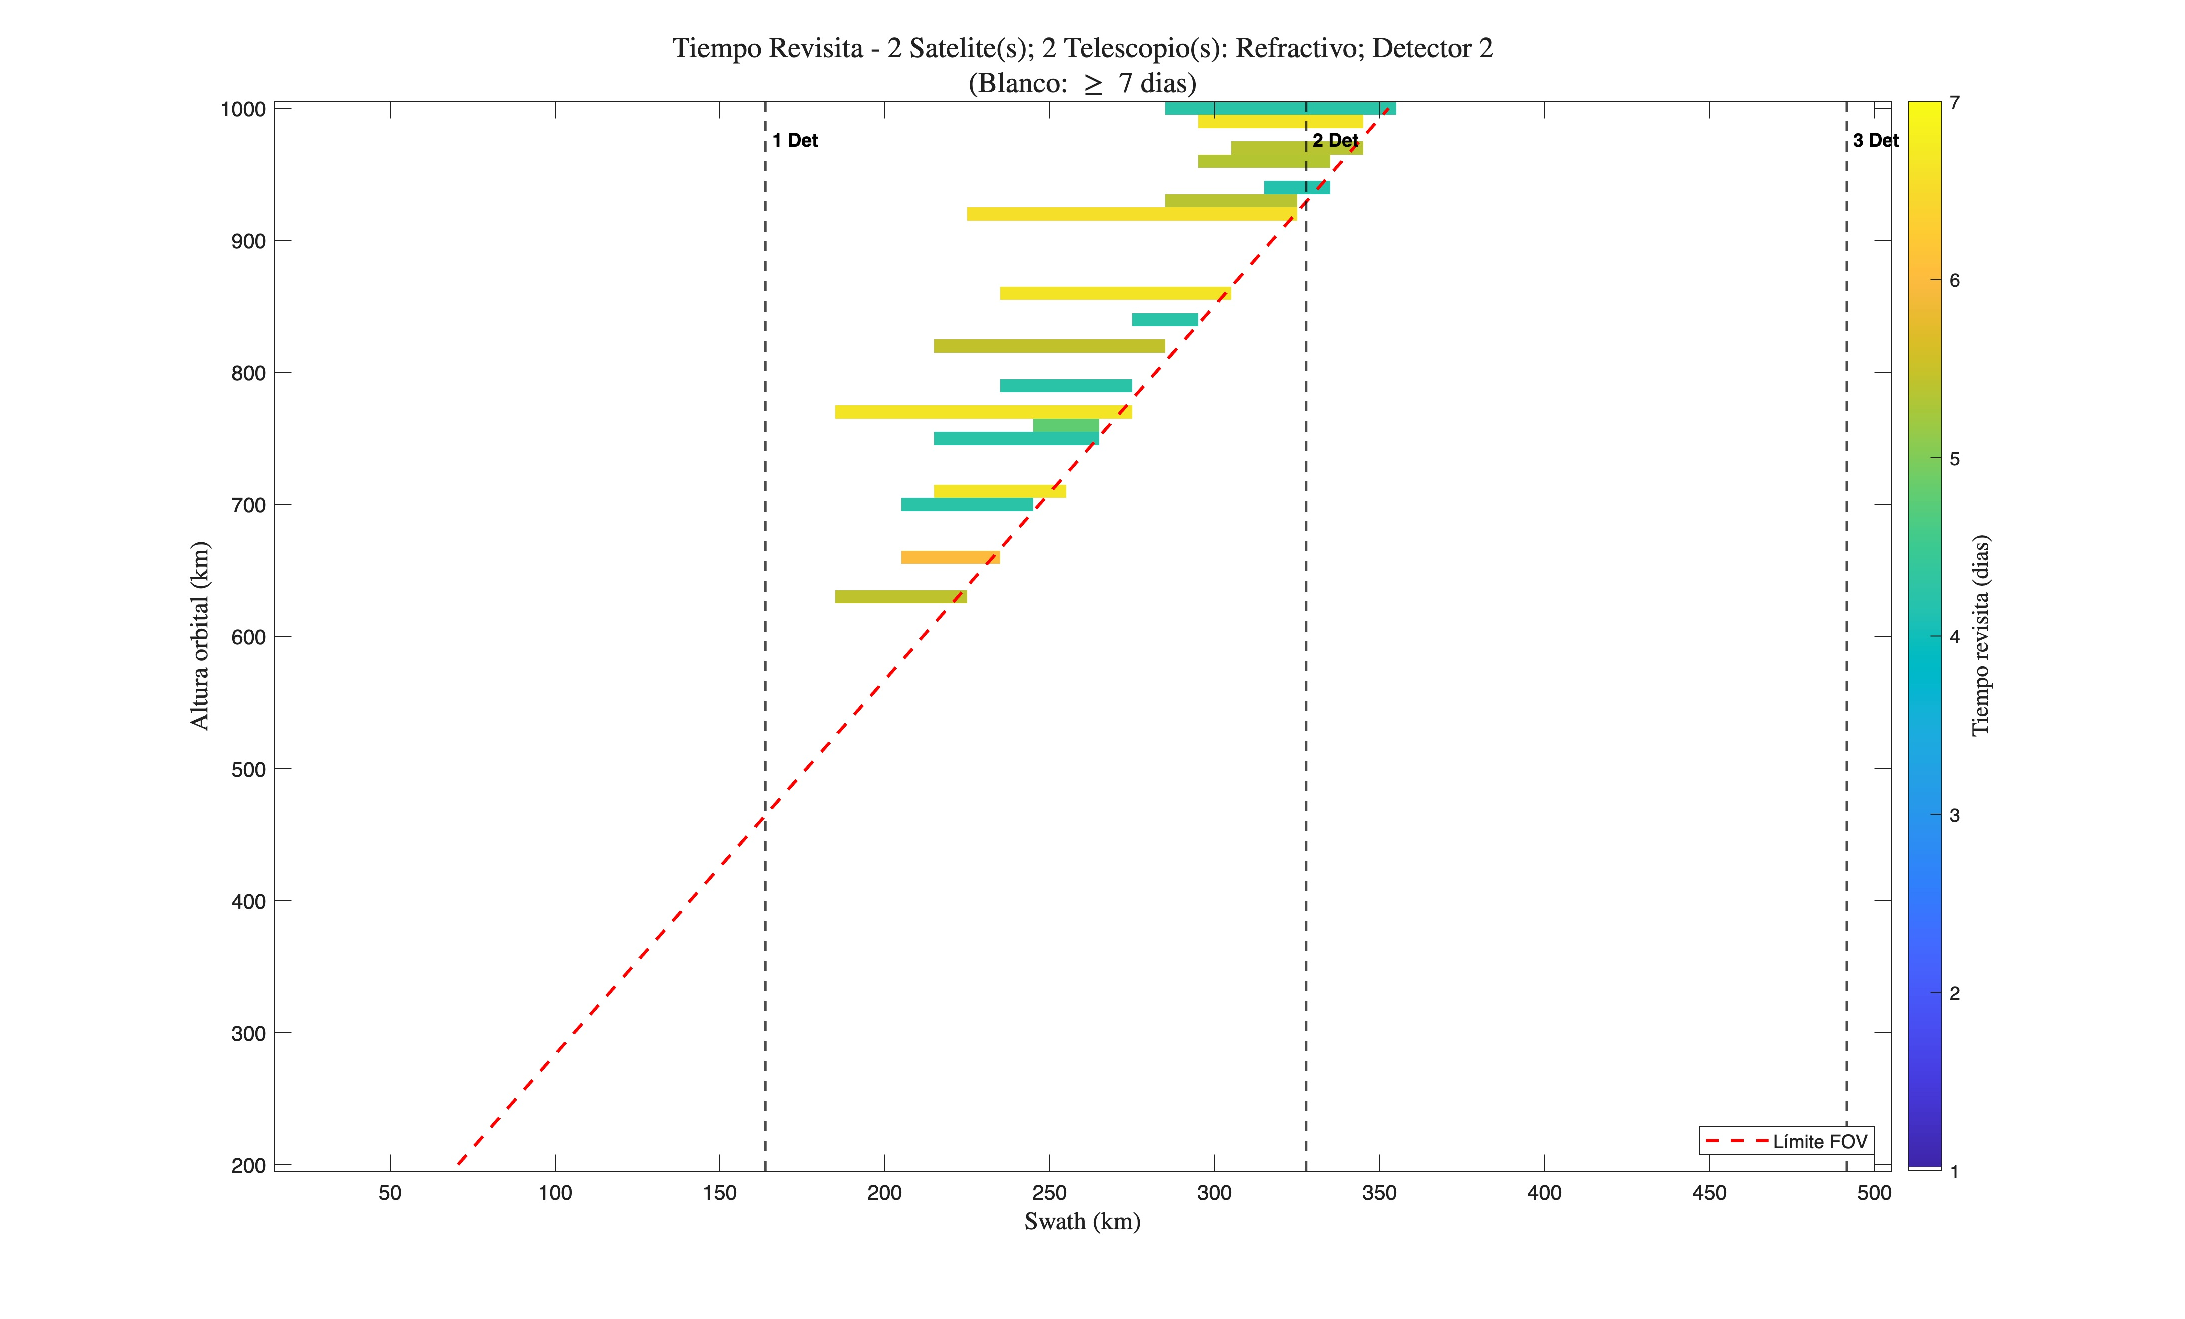
\includegraphics[width=12cm]{coverage_selected_heatmap.pdf}};

    % 2. Definir un sistema de coordenadas relativo a la imagen para facilitar la colocación
    %    El origen (0,0) es la esquina inferior izquierda.
    %    El punto (1,1) es la esquina superior derecha.
    \begin{scope}[x={(image.south east)}, y={(image.north west)}]


            
        \coordinate (PuntoDiseno) at (0.385, 0.545);

        % 4. Dibujar el punto rojo en las coordenadas definidas
        \fill[red] (PuntoDiseno) circle (2pt);
        
        % 5. Crear la caja de texto (label) y una flecha apuntando al punto
        %    El nodo se posiciona relativo al punto para que sea fácil de mover.
        \node[fill=white, draw, thick, anchor=south west, inner sep=2pt] (label) 
            at ([xshift=10pt, yshift=10pt]PuntoDiseno) {Punto de diseño};
            \draw[->, thick, -latex] (label.south west) -- (PuntoDiseno);
        % Dibuja una línea/flecha desde la caja de texto al punto
        

        

    \end{scope}

\end{tikzpicture}


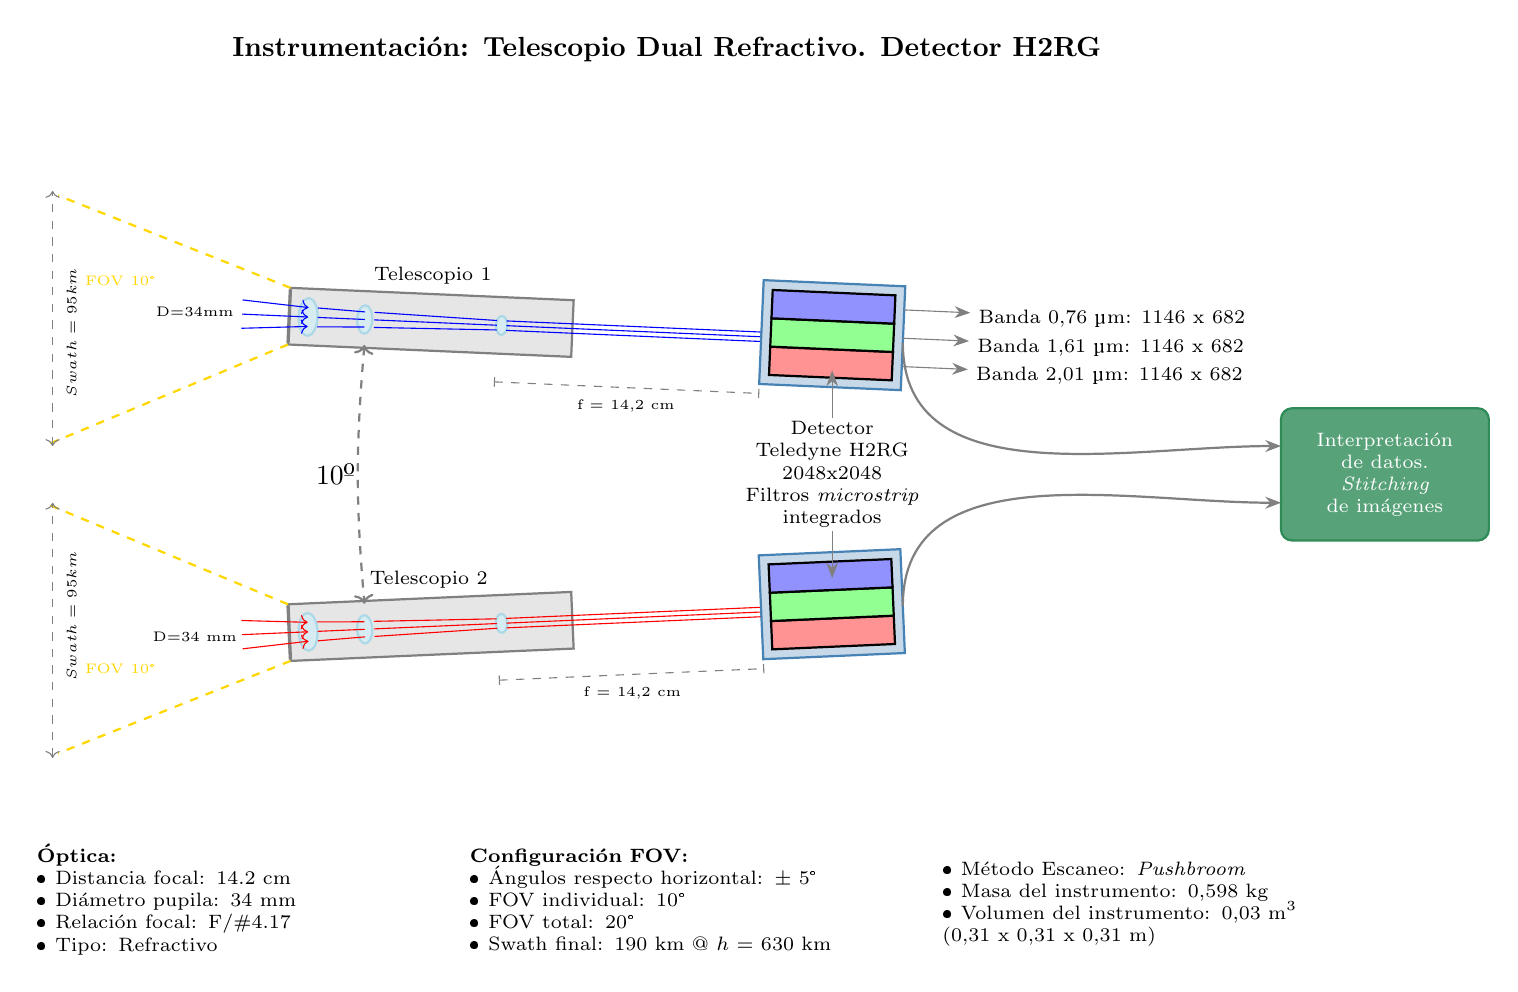
\begin{tikzpicture}[scale=1.2]
    % --- Definición de colores ---
    \definecolor{lens}{RGB}{173, 216, 230}
    \definecolor{detector}{RGB}{70, 130, 180}
    \definecolor{band1}{RGB}{255, 100, 100}
    \definecolor{band2}{RGB}{100, 255, 100}
    \definecolor{band3}{RGB}{100, 100, 255}
    \definecolor{housing}{RGB}{128, 128, 128}
    \definecolor{fov}{RGB}{255, 215, 0}
    \definecolor{microchip}{RGB}{46, 139, 87}

    % ===================================================
    % Sistema 1 (Inclinado -2.5 grados)
    % ===================================================
    \begin{scope}[yshift=1.5cm, rotate=-2.5]
        \draw[housing, thick, fill=housing!20] (-4, -0.3) rectangle (-1, 0.3);
        \node[font=\scriptsize] at (-2.5, 0.5) {Telescopio 1};
        \draw[housing, very thick] (-4, -0.28) -- (-4, 0.28);
        \node[font=\tiny] at (-5, 0) {D=34mm};
        
        \draw[lens, thick, fill=lens!50] (-3.8, 0) ellipse (0.1 and 0.2);
        \draw[lens, thick, fill=lens!50] (-3.2, 0) ellipse (0.08 and 0.15);
        \draw[lens, thick, fill=lens!50] (-1.75, 0) ellipse (0.06 and 0.1);
        
        \draw[gray, dashed] (-1.8, -0.6) -- (1, -0.6);
        \draw[gray] (-1.8, -0.65) -- (-1.8, -0.55);
        \draw[gray] (1, -0.65) -- (1, -0.55);
        \node[font=\tiny] at (-0.4, -0.8) {f = 14,2 cm};
        
        % --- RAYOS DE LUZ  (Sistema 1) ---
        \draw[blue, ->] (-4.5, 0.15) -- (-3.8, 0.1);
        \draw[blue, ->] (-4.5, 0) -- (-3.8, 0);
        \draw[blue, ->] (-4.5, -0.15) -- (-3.8, -0.1);
        \draw[blue] (-3.7, 0.1) -- (-3.2, 0.08);
        \draw[blue] (-3.7, 0) -- (-3.2, 0);
        \draw[blue] (-3.7, -0.1) -- (-3.2, -0.08);
        \draw[blue] (-3.1, 0.08) -- (-1.8, 0.05);
        \draw[blue] (-3.1, 0) -- (-1.8, 0);
        \draw[blue] (-3.1, -0.08) -- (-1.8, -0.05);
        \draw[blue] (-1.7, 0.05) -- (1, 0.05);
        \draw[blue] (-1.7, 0) -- (1, 0);
        \draw[blue] (-1.7, -0.05) -- (1, -0.05);
        
        \draw[detector, thick, fill=detector!30] (1, -0.5) rectangle (2.5, 0.6);
        
        \draw[thick, fill=band1!70] (1.1, -0.4) rectangle (2.4, -0.1);
        \draw[thick, fill=band2!70] (1.1, -0.1) rectangle (2.4, 0.2);
        \draw[thick, fill=band3!70] (1.1, 0.2) rectangle (2.4, 0.5);

        \node[font=\scriptsize, align=left] at (4.7, 0.35) {Banda 0,76 \textmu m: 1146 x 682};
        \draw[gray, -{Stealth[length=2mm]}] (2.5, 0.35) -- (3.2, 0.35);
        \node[font=\scriptsize, align=left] at (4.7, 0.05) {Banda 1,61 \textmu m: 1146 x 682};
        \draw[gray, -{Stealth[length=2mm]}] (2.5, 0.05) -- (3.2, 0.05);
        \node[font=\scriptsize, align=left] at (4.7, -0.25) {Banda 2,01 \textmu m: 1146 x 682};
        \draw[gray, -{Stealth[length=2mm]}] (2.5, -0.25) -- (3.2, -0.25);

        \draw[fov, thick, dashed] (-4, 0.3) -- (-6.5, 1.17);
        \draw[fov, thick, dashed] (-4, -0.3) -- (-6.5, -1.47);
        \node[fov, font=\tiny] at (-5.8, 0.3) {FOV 10°};

        \coordinate (D1) at (2.5, 0);
        \coordinate (C1_axis) at (0, 0);
    \end{scope}
    
    % ===================================================
    % Sistema 2 (Inclinado +2.5 grados)
    % ===================================================
    \begin{scope}[yshift=-1.5cm, rotate=2.5]
        \draw[housing, thick, fill=housing!20] (-4, -0.3) rectangle (-1, 0.3);
        \node[font=\scriptsize] at (-2.5, 0.5) {Telescopio 2};
        \draw[housing, very thick] (-4, -0.28) -- (-4, 0.28);
        \node[font=\tiny] at (-5, 0) {D=34 mm};
        
        \draw[lens, thick, fill=lens!50] (-3.8, 0) ellipse (0.1 and 0.2);
        \draw[lens, thick, fill=lens!50] (-3.2, 0) ellipse (0.08 and 0.15);
        \draw[lens, thick, fill=lens!50] (-1.75, 0) ellipse (0.06 and 0.1);
        
        \draw[gray, dashed] (-1.8, -0.6) -- (1, -0.6);
        \draw[gray] (-1.8, -0.65) -- (-1.8, -0.55);
        \draw[gray] (1, -0.65) -- (1, -0.55);
        \node[font=\tiny] at (-0.4, -0.8) {f = 14,2 cm};
        
        % --- RAYOS DE LUZ RESTAURADOS (Sistema 2) ---
        \draw[red, ->] (-4.5, 0.15) -- (-3.8, 0.1);
        \draw[red, ->] (-4.5, 0) -- (-3.8, 0);
        \draw[red, ->] (-4.5, -0.15) -- (-3.8, -0.1);
        \draw[red] (-3.7, 0.1) -- (-3.2, 0.08);
        \draw[red] (-3.7, 0) -- (-3.2, 0);
        \draw[red] (-3.7, -0.1) -- (-3.2, -0.08);
        \draw[red] (-3.1, 0.08) -- (-1.8, 0.05);
        \draw[red] (-3.1, 0) -- (-1.8, 0);
        \draw[red] (-3.1, -0.08) -- (-1.8, -0.05);
        \draw[red] (-1.7, 0.05) -- (1, 0.05);
        \draw[red] (-1.7, 0) -- (1, 0);
        \draw[red] (-1.7, -0.05) -- (1, -0.05);
        
        \draw[detector, thick, fill=detector!30] (1, -0.5) rectangle (2.5, 0.6);
        
        \draw[thick, fill=band1!70] (1.1, -0.4) rectangle (2.4, -0.1);
        \draw[thick, fill=band2!70] (1.1, -0.1) rectangle (2.4, 0.2);
        \draw[thick, fill=band3!70] (1.1, 0.2) rectangle (2.4, 0.5);

        \draw[fov, thick, dashed] (-4, 0.3) -- (-6.5, 1.47);
        \draw[fov, thick, dashed] (-4, -0.3) -- (-6.5, -1.17);
        \node[fov, font=\tiny] at (-5.8, -0.3) {FOV 10°};

        \coordinate (D2) at (2.5, 0);
        \coordinate (C2_axis) at (0, 0);
    \end{scope}

    % --- Indicador de ángulo ---
    \draw[<->, gray, dashed, thick] (-3.2,1.37) to[bend right=5] (-3.2,-1.37);
    \node at (-3.5,0) {10º};
    \draw[<->, gray, dashed] (-6.5, -3) to (-6.5, -0.3);
    \node[font=\tiny, rotate=90] at (-6.3, -1.5) {$Swath = 95 km$};
    \draw[<->, gray, dashed] (-6.5, 0.3) to (-6.5, 3);
    \node[font=\tiny, rotate=90] at (-6.3, 1.5) {$Swath = 95 km$};
    
    % --- Microcontrolador ---
    \begin{scope}[xshift=6.5cm, yshift=0cm]
        \draw[microchip, thick, fill=microchip!80, rounded corners] (0, -0.7) rectangle (2.2, 0.7);
        \node[white, font=\scriptsize, align=center, text width=2cm] at (1.1, 0) {Interpretación de datos.\\ \textit{Stitching} de imágenes};
        \coordinate (MCU_in1) at (0, 0.3);
        \coordinate (MCU_in2) at (0, -0.3);
    \end{scope}
    
    \draw[-{Stealth[length=2mm]}, thick, gray] (D1) to[out=270, in=180] (MCU_in1);
    \draw[-{Stealth[length=2mm]}, thick, gray] (D2) to[out=90, in=180] (MCU_in2);

    % --- Etiqueta del detector ---
    \node[font=\scriptsize, align=center, text width=2.5cm] at (1.75, 0) {Detector \\ Teledyne H2RG \\ 2048x2048\\Filtros \textit{microstrip} integrados};
    \draw[-{Stealth[length=2mm]}, gray] (1.75, 0.6) -- (1.75, 1.1);
    \draw[-{Stealth[length=2mm]}, gray] (1.75, -0.6) -- (1.75, -1.1);
    
    % ===================================================
    % Información y Título
    % ===================================================
    \node[font=\large, font=\bfseries] at (0, 4.5) {Instrumentación: Telescopio Dual Refractivo. Detector H2RG};
    
    \node[font=\scriptsize, align=left, text width=4cm] at (-5, -4.5) {
        \textbf{Óptica:}\\
        • Distancia focal: 14.2 cm\\
        • Diámetro pupila: 34 mm\\
        • Relación focal: F/\#4.17\\
        • Tipo: Refractivo
    };
    
    \node[font=\scriptsize, align=left, text width=5cm] at (0, -4.5) {
        \textbf{Configuración FOV:}\\
        • Ángulos respecto horizontal: $\pm$ 5° \\
        • FOV individual: 10°\\
        • FOV total: 20°\\
        • Swath final: 190 km @ $h$ = 630 km \\
    };
    \node[font=\scriptsize, align=left, text width=5cm] at (5, -4.5) {
        \textbf{ }\\
        • Método Escaneo: \textit{Pushbroom}\\
        • Masa del instrumento: 0,598 kg\\
        • Volumen del instrumento: 0,03 m\textsuperscript{3} (0,31 x 0,31 x 0,31 m)
    };

    
\end{tikzpicture}

\end{document}
